%%%%%%%%%%%%%%%%%%%%%%%%%%%%%%%%%%%%%%%%%%%%%%%%%%%%%%%%%%%%%%%%%%%%%%%%%
% $Id$
% %%%%%%%%%%%%%%%%%%%%%%%%%%%%%%%%%%%%%%%%%%%%%%%%%%%%%%%%%%%%%%%%%%%%%%%%%
%
% Set de slides dedicadas a formulacion Ewald con 1D periodicity
%
% %%%%%%%%%%%%%%%%%%%%%%%%%%%%%%%%%%%%%%%%%%%%%%%%%%%%%%%%%%%%%%%%%%%%%%%%%


    \begin{frame}[fragile,allowframebreaks]{\GreenTEw}

    
    \begin{block}{Ewald Method in HOFEM}
    \begin{columns}[T]
      \column{0.50\textwidth}
      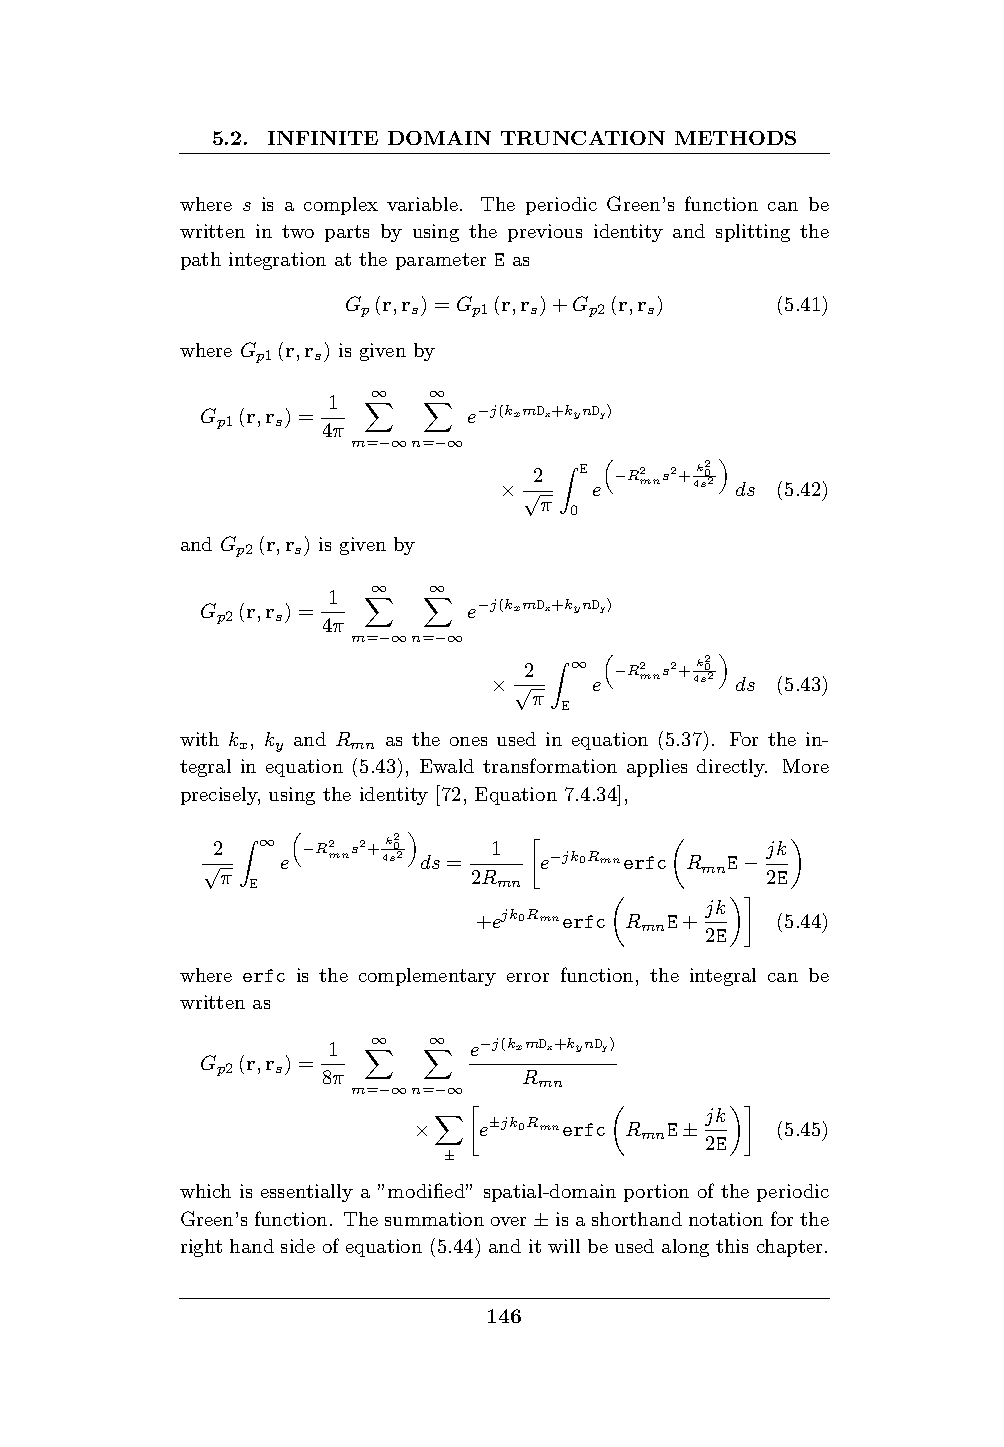
\includegraphics[width=\textwidth,clip=true,trim=70 350 70 80]{Tesis_Daniel_Ewald_1} 
      \column{0.45\textwidth}
      \begin{lstlisting}[style=myFORTRANcodeS,basicstyle=\ttfamily\tiny]
!Distancia de la celda unidad en X
 Dx = SQRT(DOT_PRODUCT(PBC_structure%offset_vector(1,:),PBC_structure%offset_vector(1,:)))
 !Distancia de la celda unidad en Y
 Dy = SQRT(DOT_PRODUCT(PBC_structure%offset_vector(2,:),PBC_structure%offset_vector(2,:)))
    
 E = SQRT(PI/Dx/Dy)

 !Sum using Ewald transformation
 DO m=-2,2
    DO n=-2,2

    !Calcular alpha_mn
    alpha_mn = SQRT(CMPLX((PI*m/Dx)**2 + (PI*n/Dy)**2 + (PI*m/Dx)*Kx + &
    (PI*n/Dy)*Ky + (1.0_DBL/4.0_DBL)*(Kx**2+Ky**2-K**2),0.0_DBL,KIND=DBL));
      \end{lstlisting}
    \end{columns}
  \end{block}


  \begin{block}{Ewald 1D periodicity}
    \begin{itemize}
    \item Naively we thought if was simply setting
      either $m=0$ or $n=0$
    \item \alert{But it is NOT} \ldots
%      \hyperlink{Ewald1D}{click here to go to section on Ewald 1D}
      \hyperlink{Ewald1D}{see next slided on Ewald 1D}
    \end{itemize}
  \end{block}

  \end{frame}

  % %%%%%%%%%%%%%%%%%%%%%%%%%%%%%%%%%%%%%%%%%%%%%%%%%%%%%%%%%%%%%%%
  
\begin{frame}[allowframebreaks]{Ewald sum}

  \begin{itemize}
    \item Technique for summing contribution from an infinite set of sources (in 
      this case along $z$ axis):
      \[
        \sum_n G(R_n) = 
        \frac{1}{4\pi}\sum_n
        e^{-j(k\cos\theta)nd}
        \frac{e^{-jkR_n}}{R_n}
      \]
      \small
      where 
      $R_n=\sqrt{(x-x')^2 + (y-y')^2 + (z-z'+nd)^2}$, $\theta$ is elevation 
      angle.
    \item The Green function is decomposed in two terms:
      \[
        \sum_n G(R_n) = \sum_n G_1(R_n) + \sum_n G_2(R_n)
      \]
      \begin{itemize}
        \item One of them decays quickly with $R_n$: $|G_2(R_{n+1})| \ll |G_2(R_{n})|$
        \item For the other one the 
          \href{https://en.wikipedia.org/wiki/Poisson_summation_formula}
          {Poisson summation formula}
          is applied:
          \[
            \sum_n G_1(R_n) = \sum_n \hat{G}_1(k_n)
          \]

          \vspace{-2ex}
          where $\hat{G}_1(k)$ is the Fourier transform of $G_1(R)$%
          \footnote{$\hat{G}_1(k)$ is narrow in $k$ because $G_1(R)$ is wide in $R$}.

      \end{itemize}

  \end{itemize}

  
\end{frame}
  
% %%%%%%%%%%%%%%%%%%%%%%%%%%%%%%%%%%%%%%%%%%%%%%%%%%%%%%%%%%%%%%%

\begin{frame}[allowframebreaks]{1D from 2D periodicity Ewald sum}

  \begin{itemize}
    \item No problem with \emph{spatial} term:
      \[
        \sum_m\sum_n G_2(R_{n,m}) \rightarrow \sum_{n} G_2(R_{n,0})
      \]
    \item But the \emph{spectral} term...
      \[
        \sum_m\sum_n \hat{G}_1(k_{n,m}) \rightarrow ??
      \]

      The Fourier Transform of $G_1(n,0)$ must be computed from scratch:

      \begin{gather*}
        \hat{G}_{1,n} =
        \frac{e^{j(z-z')(k_z - 2\pi \frac{n}{d})}}{2 \pi d} 
        g\left(\frac{\alpha_n^2}{4 E^2}, \rho^2 E^2\right)
        \\
         \rho^2 = (x-x')^2 + (y-y')^2
         \qquad
         \alpha_n^2 = \left(k\cos\theta + \frac{2 \pi n}{d}\right)^2 - k^2
      \end{gather*}
      where we need the following numerical integration
      \[
        g(a,b) = \int_0^1 \frac{
          e^{-\frac{a}{z^2}-b z^2}
        }{z}
        \, dz
      \]
  \end{itemize}

\end{frame}

% %%%%%%%%%%%%%%%%%%%%%%%%%%%%%%%%%%%%%%%%%%%%%%%%%%%%%%%%%%%%%%%

\begin{frame}[allowframebreaks]{Notes about g(a,b)}
  \begin{itemize}
    \item It is a complex integral whose value (and convergence) depends on the chosen path.
    \item For calculating $\hat{G}_{1,n}$:
      \begin{itemize}
        \item $a,b \in \mathbb{R}$
        \item $b>0$, 
        \item but $a$ is negative for the first $n$ values (At each $n$ term in 
          the sum $a=\alpha_n^2/4E^2$).
      \end{itemize}
    \item If $a>0$, the integral can be done through real axis.
    \item If $a<0$, the integral must be done through the following path:

      \vbs

      \usetikzlibrary {arrows.meta}
      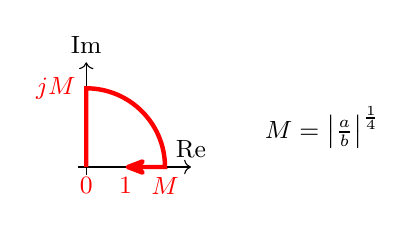
\begin{tikzpicture}[node font=\small]
        \draw[->] (-0.1,0) -- (1.33,0) node[above] {Re};
        \draw[->] (0,-0.1) -- (0,1.33) node[above] {Im};
        \draw[red, ultra thick, arrows={-Stealth[round]}] 
          (0,0) node [below] {$0$} -- (0,1) node[left] {$jM$} 
        arc[start angle=90, end angle=0, radius=1] node[below] {$M$}
        -- (0.5,0) node[below] {$1$}
        ;
        \node at (3,0.5) {$M=\left|\frac{a}{b}\right|^{\frac{1}{4}}$};
      \end{tikzpicture}

    \item If $a=0$, integral does not converge. It happens for specific values 
      of $k$ and $d$ (not a problem: Greens function is singular there).
  \end{itemize}
\end{frame}

% %%%%%%%%%%%%%%%%%%%%%%%%%%%%%%%%%%%%%%%%%%%%%%%%%%%%%%%%%%%%%%%

\begin{frame}{Checking results (thin slice)}
  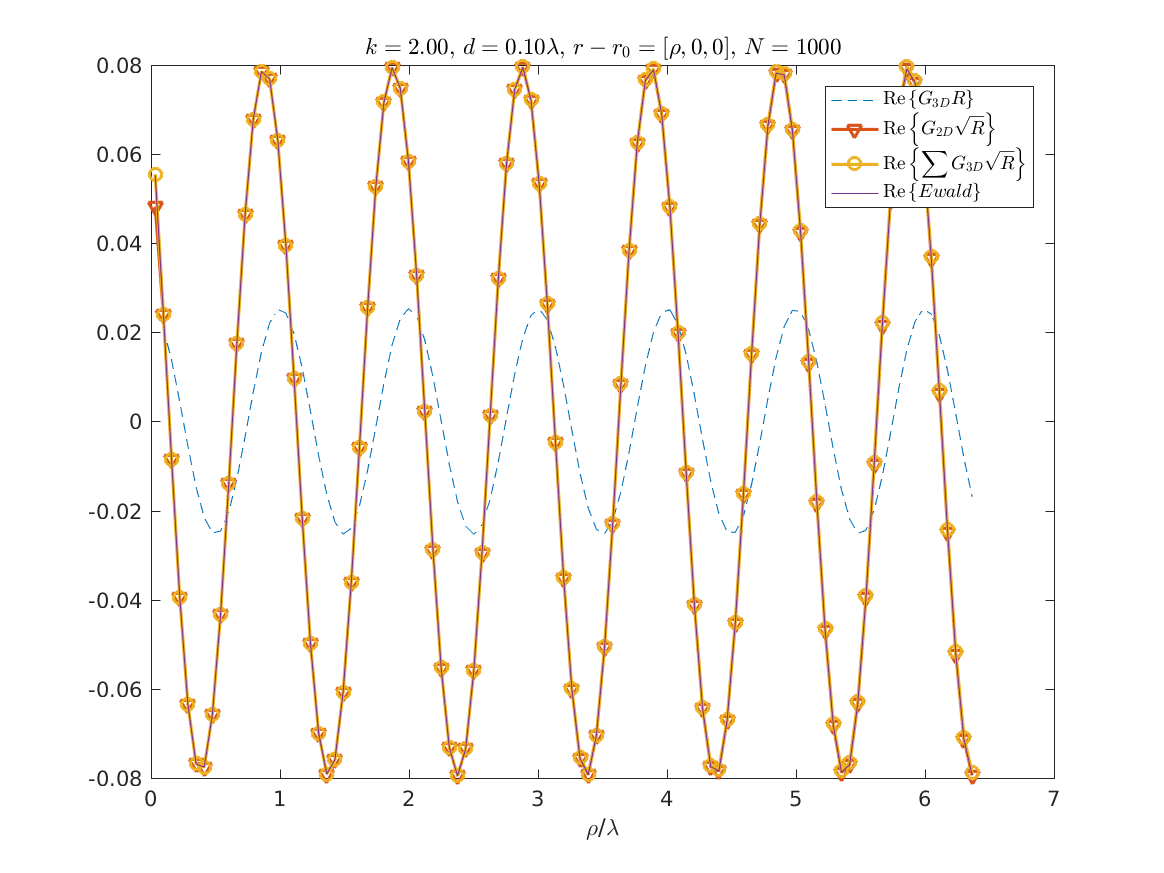
\includegraphics[width=0.9\textwidth]{GreenFunctions_R_ew1.png}
\end{frame}
\begin{frame}{Checking results (medium slice)}
  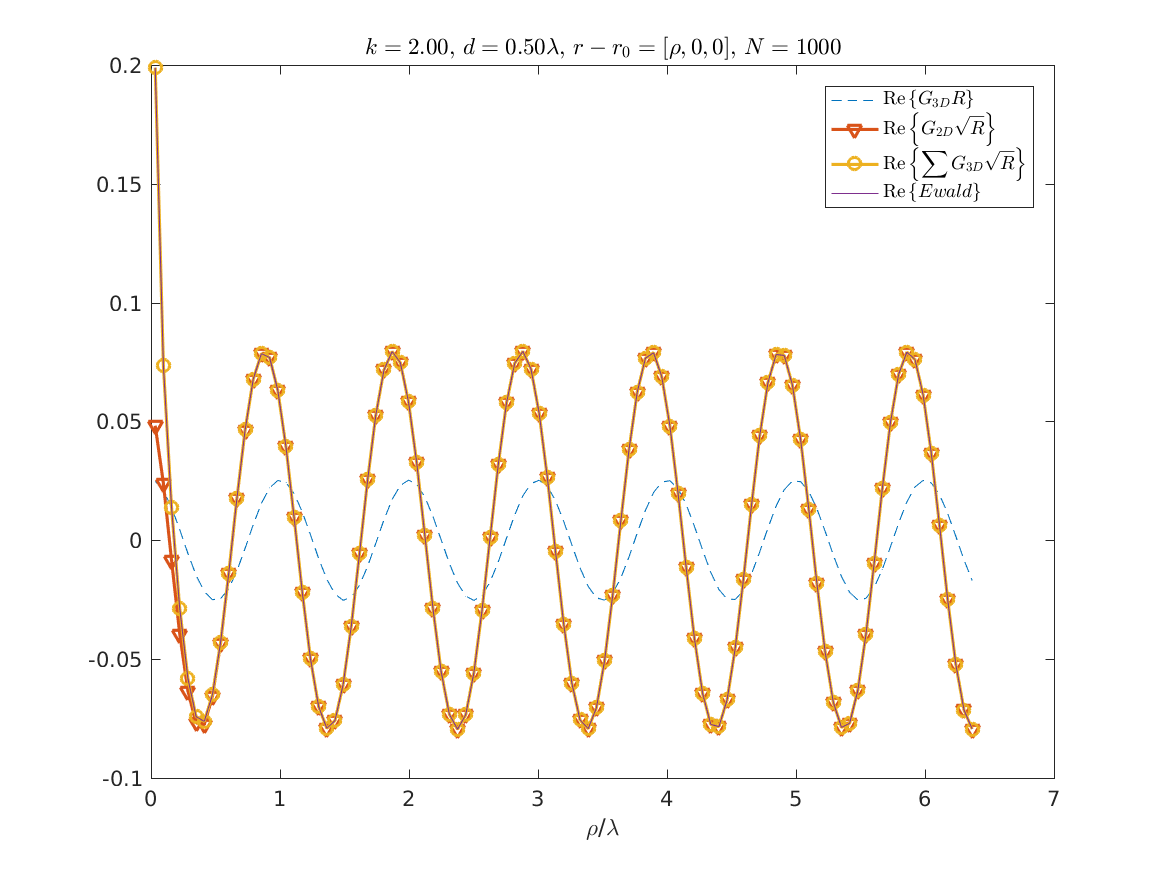
\includegraphics[width=0.9\textwidth]{GreenFunctions_R_ew2.png}
\end{frame}
\begin{frame}{Checking results (thick slice)}
  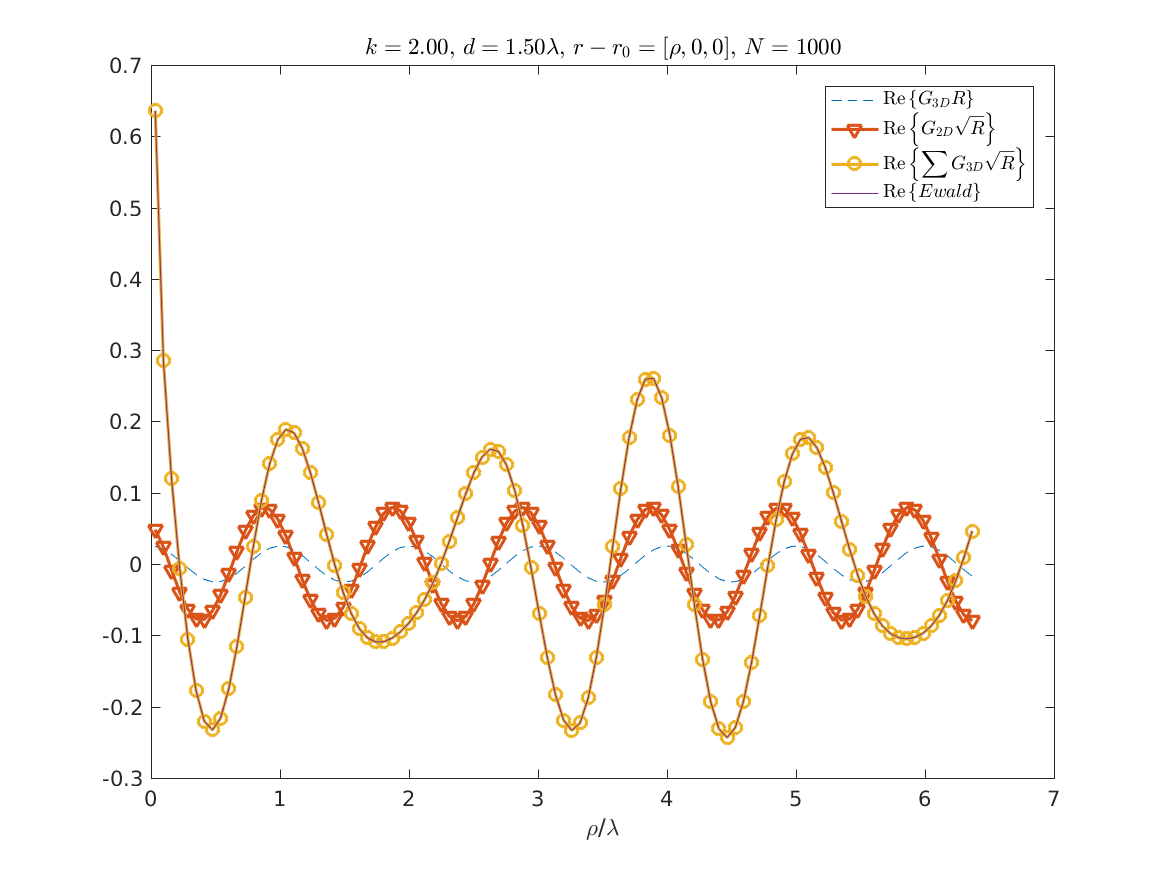
\includegraphics[width=0.9\textwidth]{GreenFunctions_R_ew3.png}
\end{frame}
\begin{frame}{Checking results (close to transverse Floquet resonance)}{$\alpha^2_0 \simeq 0$}
  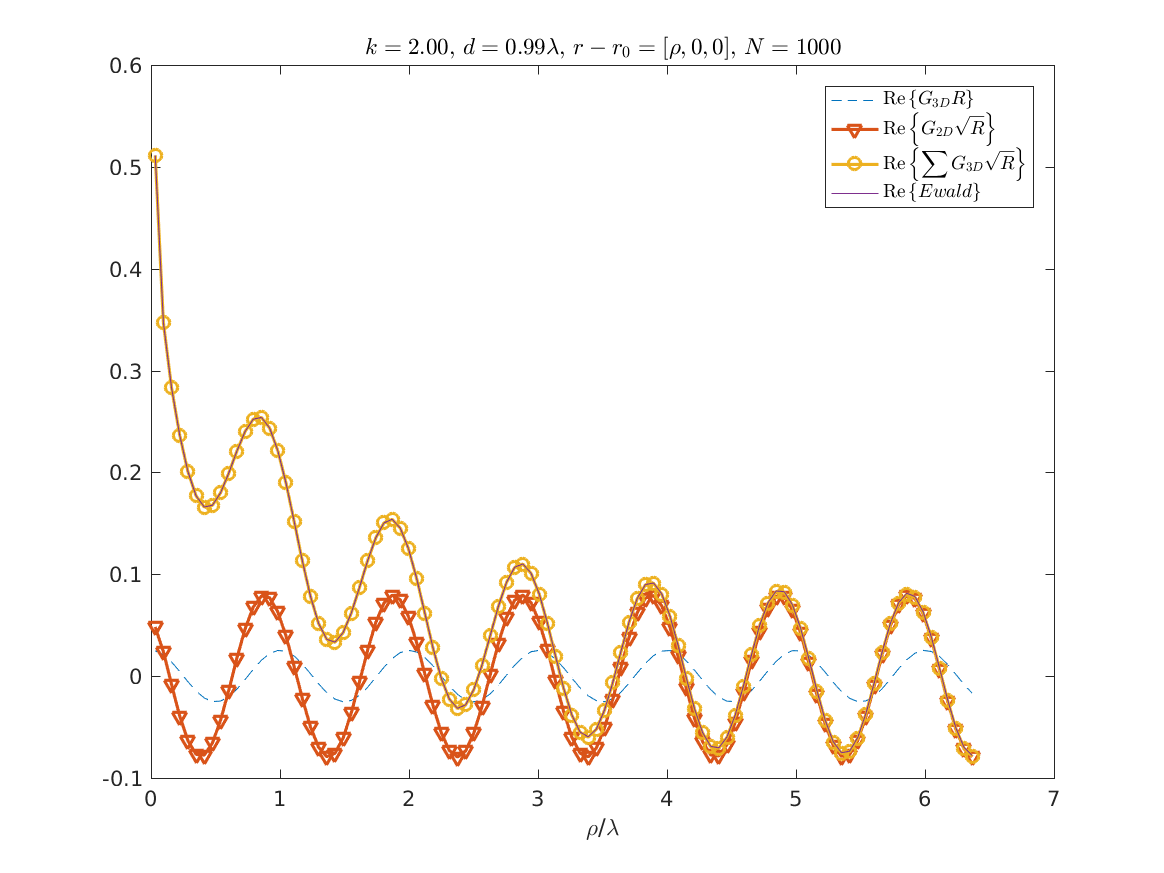
\includegraphics[width=0.9\textwidth]{GreenFunctions_R_ew_P0.png}
\end{frame}
\begin{frame}{Checking results (close to transverse Floquet 
  resonance)}{$\alpha^2_0 \simeq 0$}
  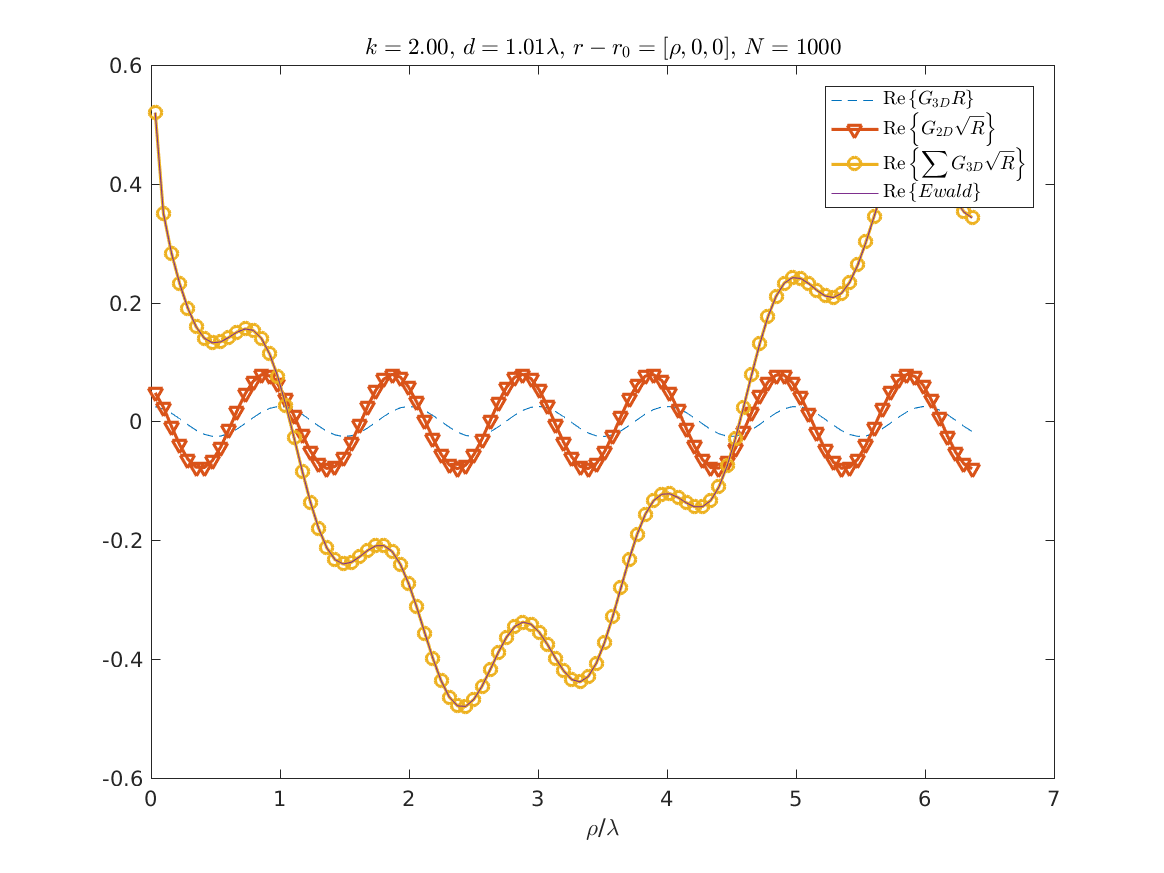
\includegraphics[width=0.9\textwidth]{GreenFunctions_R_ew_P1.png}
\end{frame}
\begin{frame}[allowframebreaks]{Convergence of the direct sum}

  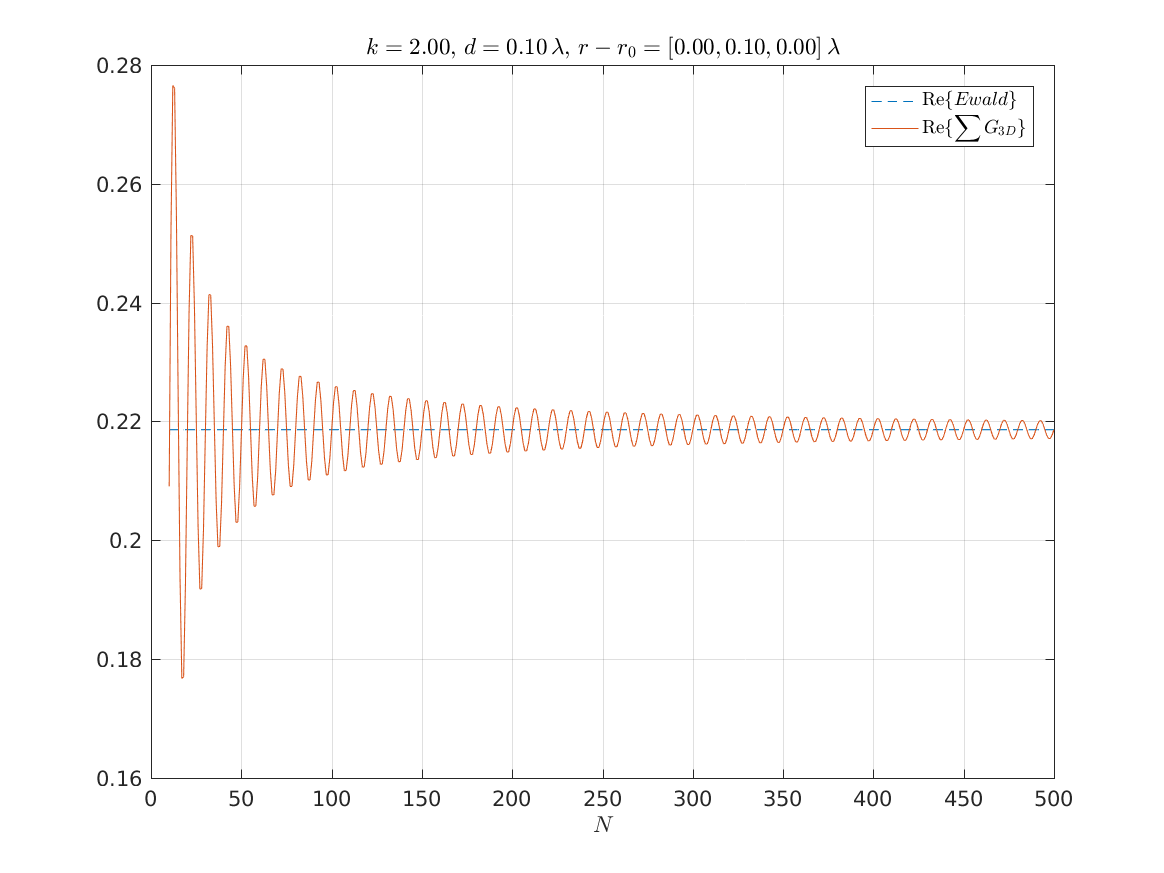
\includegraphics[width=0.8\textwidth]{GreenFunctions_convN_re_ew01.png}
 
  \framebreak

  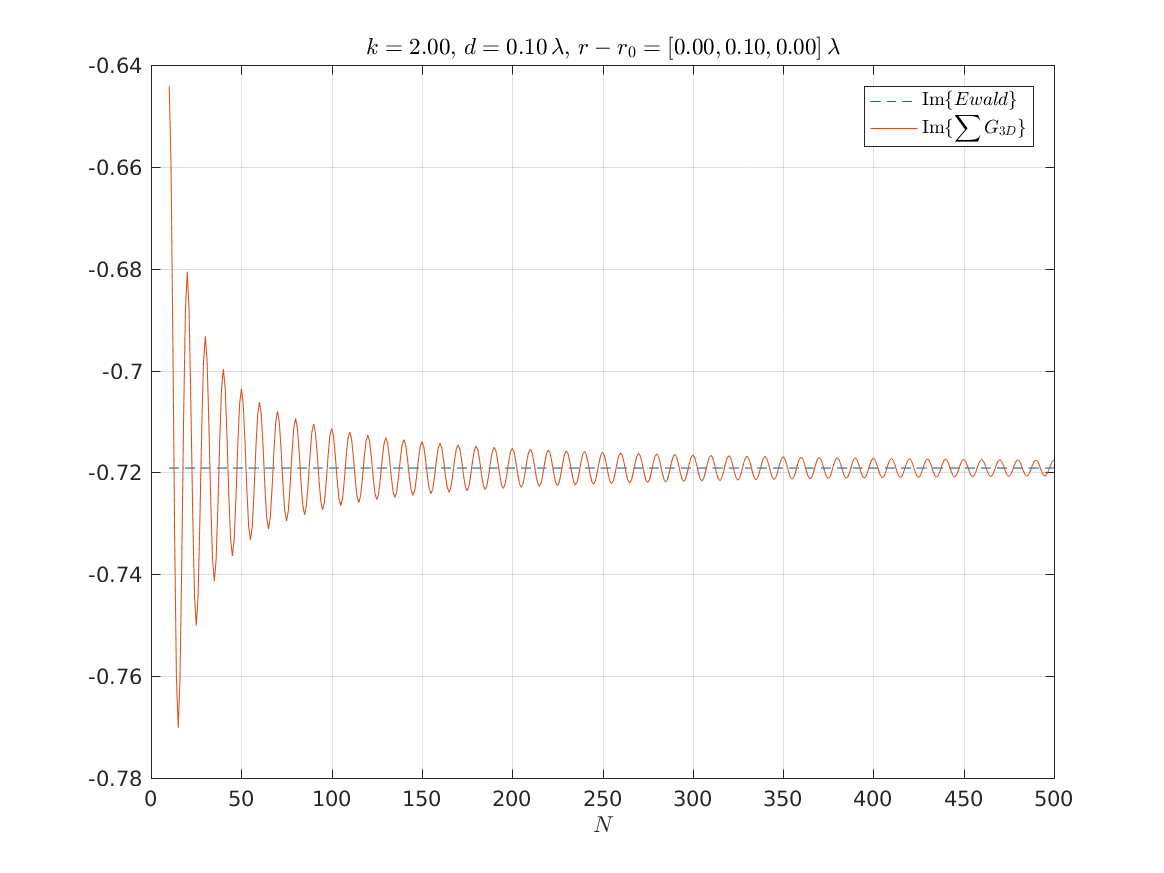
\includegraphics[width=0.8\textwidth]{GreenFunctions_convN_im_ew01.png}
\end{frame}
\begin{frame}{Dependence with frequency}
  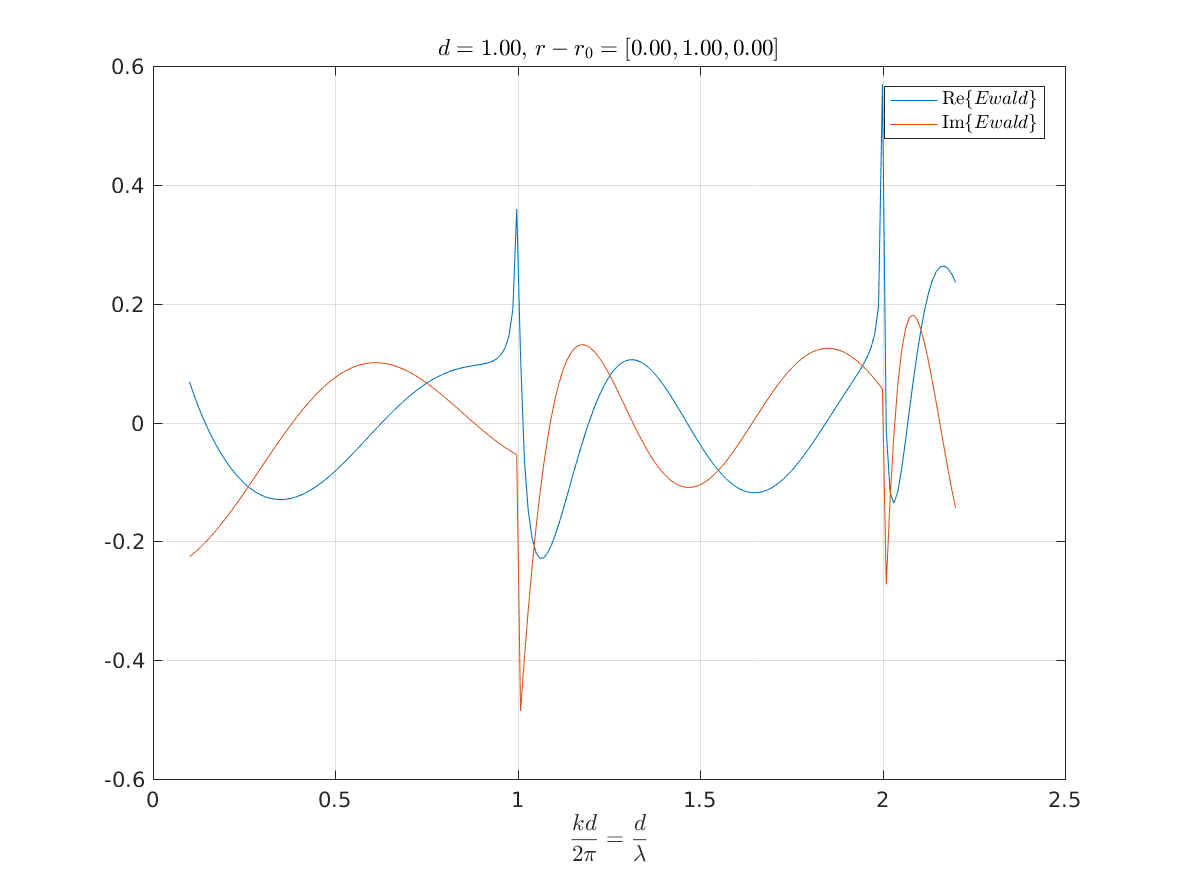
\includegraphics[width=0.9\textwidth]{GreenFunctions_ewald_k.png}
\end{frame}
\begin{frame}{Singularities when $\alpha_n^2 \to 0$}
  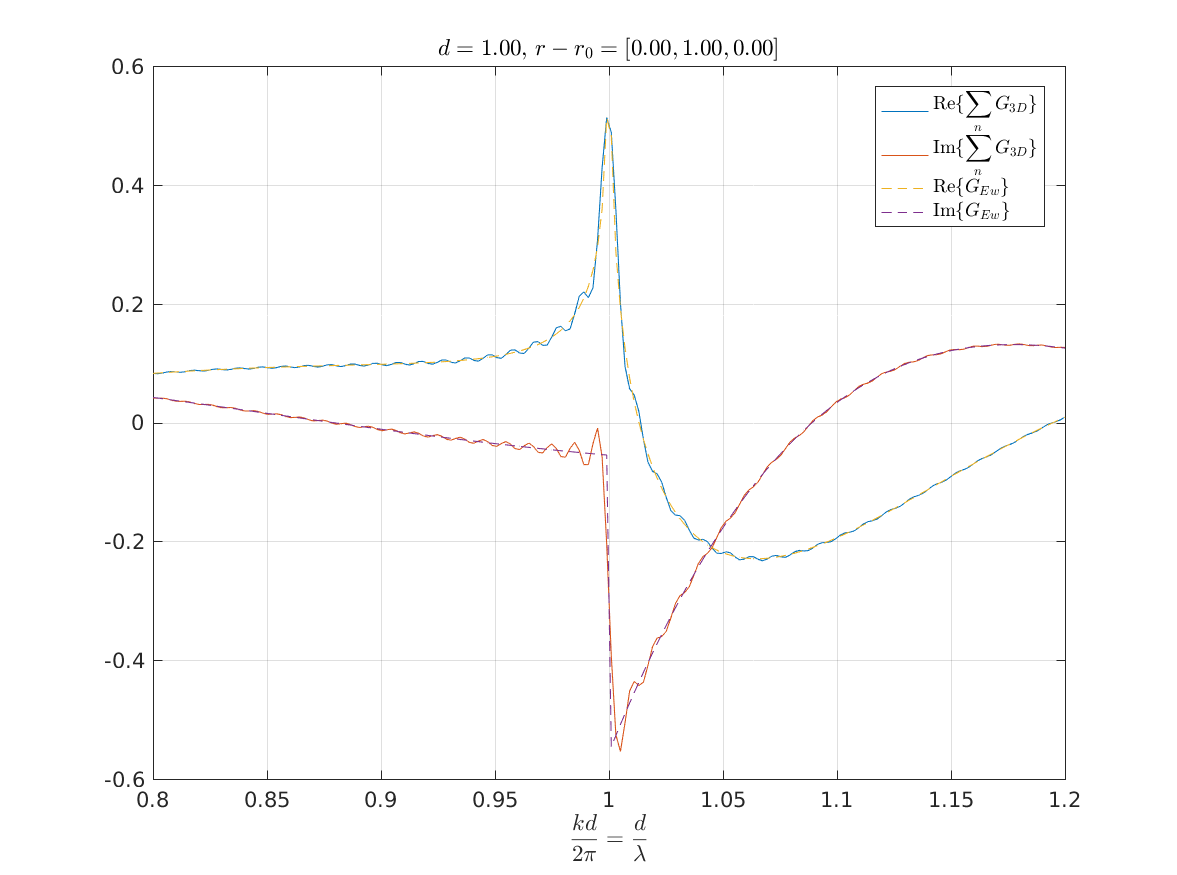
\includegraphics[width=0.9\textwidth]{GreenFunctions_ewald_k2.png}
\end{frame}

\begin{frame}{Additional notes}
  \begin{itemize}
    \item CPU time cost similar to sum 100 terms of $G_{3D}$.
    \item Matlab prototype.
    \item Numerical integral may be improved using classic algorithms for 
      calculate exponential integrals (see %
        \footnote{
          F. Capolino \emph{et al.}, ``Efficient Computation of the 2-D Green's 
          Function for 1-D Periodic Structures Using the Ewald Method'', 
          \emph{IEEE-TAP}, 2005. Equation (23).
        } and
        \footnote{
          F. Capolino \emph{et al.}, ``Efficient Computation of the 3D Green's 
          Function with One Dimensional Periodicity Using the Ewald Method'', 
          \emph{IEEE-APS}, 2006.
        })
      {\color{red} Done!: Calculation 10 times faster, but inestable for large 
      values of $\rho$ ($\rho>d$)}
    \item
      Checked:

      \[
        \int_{-\frac{d}{2}}^{\frac{d}{2}}
        G_{3D}(\rho,z)\, dz
        =
        G_{2D}(\rho)
      \]

      where $G_{3D}$ is numerically evaluated with Ewald, and $G_{2D}$ is the 
      Hankel function: 
      $\frac{1}{4j} H_0^{(2)}(k|\rho|)$.

  \end{itemize}
\end{frame}
